\chapter{Application end}
%\chapter{Application à la Transmission d’un fichier quelconque (*.mpeg, *.mp3, *.txt, *.doc, *.pdf, etc)}

\minitoc


\section{Notions sur les formats étudiés}
\paragraph{}
Nous choisissons de décrire les deux formats que nous allons utilisés par les définitions suivantes:
\paragraph{}
PPM est un format de fichier image selon (\href{http://fr.wikipedia.org/wiki/Portable_pixmap#Fichier_binaire_3}{Wikipedia}) « Ce format de fichier est utilisé pour des images couleur. Chaque pixel est codé par trois valeurs (rouge, vert et bleu). Comme le format PGM, en plus des caractéristiques de largeur et hauteur, une valeur maximale utilisée pour coder les niveaux de couleur ; cette valeur doit être inférieure à 65536. »
Sa structuration binaire est toujours définie selon la même source comme comprenant un header pour un fichier binaire ou ASCII comme suit: « Un fichier ppm binaire a pour nombre magique P6. Chaque pixel est codé sur 1 ou 2 bytes selon que la valeur maximale soit inférieure ou supérieure à 256. » (bytes=octets) Le header est donc défini selon l'information transportée.
\paragraph{}
 	 JPEG (acronyme de Joint Photographic Experts Group) est une norme qui définit le format d'enregistrement et l'algorithme de décodage pour une représentation numérique compressée d'une image fixe. (\href{http://fr.wikipedia.org/wiki/JPEG}{Wikipedia})  

\paragraph{}
La différence entre JPEG et PPM est que le premier format utilise un codage entropique tandis que le second utilise un codage fixe pour la quantification.


\section{Transmission des fichiers}
\paragraph{}
Nous faisons transiter deux images, codées par les différents formats que nous avons précités, sur notre chaîne pour en évaluer la dégradation. Le choix de deux formats, nous permet de constater les erreurs de transmission typiques à chaque format ou du moins l'impact des erreurs de transmission sur chacun des formats(leur sensibilité). 
\clearpage
Voici les images choisies pour chaque format:

\begin{figure}[bth]%[!ht]
\begin{center}

\includegraphics[height=70mm,width=70mm]{test_jpeg}%[scale=0.45]
\caption{\textbf{Image jpg choisie}}%
\url {http://www.google.fr/}
\label{test_jpeg}%
\end {center}
\end{figure}

\begin{figure}[bth]%[!ht]
\begin{center}

\includegraphics[height=70mm,width=70mm]{test_bmp}%
\caption{\textbf{Image ppm choisie}}%
\url {http://www.google.fr/}
\label{bmp}%
\end {center}
\end{figure}


\textbf{On constate bien que les images ont une représentation différente selon chaque format. Par, exemple les dimensions (128 x 128 pour jpeg et 190 x 143 pour bmp)et tailles (14Ko pour jpeg et 10Ko pour bmp) de l'image sont différentes. En général, le codage bmp donne une image plus lourde car il s'agit d'un codage fixe, la conversion de l'une ou l'autre de ces images, nous aurait permis de vérifier cela. Ceci s'explique également par le fait que chaque représentation de format est inextricablement liée au codage qui lui est propre.}

\paragraph{}
Notons que pour atténuer l'erreur de transmission, nous augmentons le paramètre AddNDensity du générateur de bruit. Nous présentons dans ces différentes sections, nos résultats de transmission obtenus.


\subsection{Transmission sans erreur}
\paragraph{}
On règle le générateur de bruit en fixant son paramètre AddNDensity à $- 65$ dB et on arrive à minimiser toute l'erreur de transmission. De cette valeur à $- 70$ dB, nous n'avons pas de dégradation et un faible taux d'erreur binaire (BER).On injecte les fichiers binaires obtenu pour chaque image puis on obtient :


\paragraph{}
Nous obtenons les images suivantes:


\begin{figure}[bth]%[!ht]
\begin{center}

\includegraphics[height=70mm,width=70mm]{test_jpeg}%
\caption{\textbf{Image jpg transmise sans erreur}}%
%\url {http://www.google.fr/}
\label{jpgsserr}%
\end {center}
\end{figure}

\paragraph{}
\begin{figure}[bth]%[!ht]
\begin{center}

\includegraphics[height=70mm,width=70mm]{BMP_test_bruit65dB}%height=70mm,width=70mm
\caption{\textbf{Image bmp transmise sans erreur}}%
%\url {http://www.google.fr/}
\label{bmpsserr}%
\end {center}
\end{figure}


\paragraph{}
Comme attendu, il n'y a d'erreur visible sur cette image. Les images sont très identiques à celles de départ. Ceci avec un BER de $9.745 * 10^ - ­6$ pour JPEG et $4.295 * 10^ - ­5$ pour BMP. Le premier étant donc plus faible.




\subsection{Transmission avec très peu d’erreurs}
\paragraph{}
En augmentant progressivement les erreurs sur notre transmission, nous obtenons les résultats suivants:



\begin{figure}[bth]%[!ht]
\begin{center}

\includegraphics[height=70mm,width=70mm]{jpg_test_bruit65dB}%
\caption{\textbf{Format JPG: Transmission avec très peu d’erreurs}}%
%\url {http://www.google.fr/}
\label{jpg_test_bruit65dB}%
\end {center}
\end{figure}

\begin{figure}[bth]%[!ht]
\begin{center}

\includegraphics[height=70mm,width=70mm]{BMP_test_bruit64dB}%
\caption{\textbf{Format PPM: Transmission avec très peu d’erreurs}}%
%\url {http://www.google.fr/}
\label{BMP_test_bruit64dB}%
\end {center}
\end{figure}
\paragraph{}
%Comme précédemment, il y a très peu de dégradations avec un un BER de  $2.824 * 10^-5$ pour JPEG et $7.158 * 10^-4$ pour BMP avec un AddNDensity à $- 64$ dB.


\subsection{Transmission avec beaucoup d’erreurs}
\paragraph{}

 A partir de -61dB pour l'image en bmp, nous arrivons pas à afficher notre image et nous avons un taux d'erreur binaire de 0.001 tandis que pour le format jpg cela apparait lorsque que le paramètre est en dessous de -60dB.

\begin{figure}[bth]%[!ht]
\begin{center}

\includegraphics[height=70mm,width=70mm]{jpg_test_bruit63dB}%
\caption{\textbf{Format JPG: Transmission avec beaucoup d’erreurs}}%
ù\url {http://www.google.fr/}
\label{jpg_test_bruit63dB}%
\end {center}
\end{figure}

\begin{figure}[bth]%[!ht]
\begin{center}
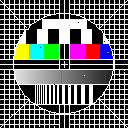
\includegraphics[height=70mm,width=70mm]{BMP_test_bruit62dB}%
\caption{\textbf{Format PPM: Transmission avec beaucoup d’erreurs}}%
%\url {http://www.google.fr/}
\label{BMP_test_bruit62dB}%
\end {center}
\end{figure}

\begin{table}[!ht]%
\begin{center}
\begin{tabular}{|c|c|c|}
\hline 
Description &AddNDensity &BER\\
\hline 
\scriptsize{JPG}&\scriptsize  {-­60dB}&\scriptsize  {$0.004$}\\
\hline
 \scriptsize{BMP} & \scriptsize {-­62dB}&\scriptsize  {$4.438*10^-4$}\\
\hline 
\end{tabular}
\end{center}
\caption{\textbf{Description du paramètre AddNDensity sur l'erreur de transmission engendrée}}
\label{tab2}
\end{table}
\paragraph{}
%Ces images sont obtenues avec un un BER de $0.004$ pour JPEG et $4.438 * 10^-4$ pour BMP avec respectivement un AddNDensity à $- 60$ dB et $- 62dB$. On remarque de fortes dégradations des images. Sur JPEG, nous avons comme des bandes qui sont désynchronisées et sur BPM des points qui marquent des erreurs.
\paragraph{}
Il faut préciser que BPM supporte un paramètre d'erreur plus élevé mais que son BER reste toujours plus faible que celui de JPEG. Toutefois, l'image est beaucoup plus visible que celle de JPEG. 

\subsection{Transmission avec peu d’erreurs}
\paragraph{}




\begin{figure}[bth]%[!ht]
\begin{center}
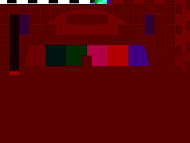
\includegraphics[height=70mm,width=70mm]{jpg_test_bruit64dB}%
\caption{\textbf{Format JPG: Transmission avec peu d’erreurs}}%
\url {http://www.google.fr/}
\label{jpg_test_bruit64dB}%
\end {center}
\end{figure}

\begin{figure}[bth]%[!ht]
\begin{center}

\includegraphics[height=70mm,width=70mm]{BMP_test_bruit63dB}%
\caption{\textbf{Format PPM: Transmission avec peu d’erreurs}}%
%\url {http://www.google.fr/}
\label{BMP_test_bruit63dB}%
\end {center}
\end{figure}

\paragraph{}
%Ces images sont obtenues avec un un BER de $1.186 * 10^-4$ pour JPEG et {$1.503 * 10^-4$} pour BMP avec un AddNDensity à $- 63$ dB. Comme dégradation, on observe un point significatif d'un pixel erronné. Il s'agit d'une erreur localisée tandis qu'en JPEG, nous avons une erreur liée aux bandes, cela montre bien que JPEG est un codage entropique et non fixe. Il est codé par bloc de 8.

\paragraph{}
De cette partie, on peut conclure que l'image à codage fixe : BPM supporte beaucoup plus les erreurs car elles restent plus visibles que JPEG. Ceci est dû au fait qu'un bit erronné dans un codage fixe ne dégrade pas tous les suivants car il est codé avec erreur et ne respectant pas le principe de préfixe, le décodage lie correctement les bits suivants. 
